% To je predloga za poročila o domačih nalogah pri predmetih, katerih
% nosilec je Blaž Zupan. Seveda lahko tudi dodaš kakšen nov, zanimiv
% in uporaben element, ki ga v tej predlogi (še) ni. Več o LaTeX-u izveš na
% spletu, na primer na http://tobi.oetiker.ch/lshort/lshort.pdf.
%
% To predlogo lahko spremeniš v PDF dokument s pomočjo programa
% pdflatex, ki je del standardne instalacije LaTeX programov.

\documentclass[a4paper,11pt]{article}
\usepackage{a4wide}
\usepackage{fullpage}
\usepackage[utf8x]{inputenc}
\usepackage[slovene]{babel}
\selectlanguage{slovene}
\usepackage[toc,page]{appendix}
\usepackage[pdftex]{graphicx} % za slike
\usepackage{setspace}
\usepackage{color}
\definecolor{light-gray}{gray}{0.95}
\usepackage{listings} % za vključevanje kode
\usepackage{hyperref}
\usepackage[]{algorithm2e}
\usepackage{program}
\usepackage[table]{xcolor}
\usepackage{float}
\usepackage{makecell}
\usepackage{multirow}
\usepackage{algpseudocode}
\renewcommand{\baselinestretch}{1.2} % za boljšo berljivost večji razmak
\renewcommand{\appendixpagename}{Priloge}

\lstset{ % nastavitve za izpis kode, sem lahko tudi kaj dodaš/spremeniš
language=Python,
basicstyle=\footnotesize,
basicstyle=\ttfamily\footnotesize\setstretch{1},
backgroundcolor=\color{light-gray},
}

\title{Modeliranje časovnih trendov z markovskimi verigami \\ \large  Poročilo izvorne kode}
\author{Jaka Kordež \\ Anže Gregorc}
\date{\today}

\begin{document}

\maketitle

\tableofcontents

\section{Uvod}

Pri predmetu bomo spoznavali sisteme za vzporedno in porazdeljeno procesiranje. Izbrali smo problem, ki ga bomo v skupinah po dva tekom semestra nadgrajevali s pomočjo različnih pristopov za paralelno programiranje. Tokrat pa je poročilo namenjeno opisu paralelizacije in meritev.

\section{Paralelizacija s Pthreads}

\subsection{Ideja paralelizacije}

Ker je glavna struktura matrika, je paralelizacijo dokaj lahko implementirati. Dogaja se pri normalizaciji matrike. Vsaka nit opravi delo na svojem kosu podatkov. Ker je matrika implementirana kot ena velika vrsta, vsaka nit dobi nalogo opraviti delo na določenem kosu le te. Z drugimi besedami, zaporedne celice v vrsti sledijo po stolpcu navzdol, torej lahko rečemo, da smo matriko razdelili po stolpcih. Komunikacija med delom niti ni potrebna, le na koncu se morajo počakati, da dokončajo in nato program začne računati uspešnost napovedi te matrike.


\begin{figure}[H]
\begin{center}
\caption{Shema glavne ideje pri paralelizaciji}
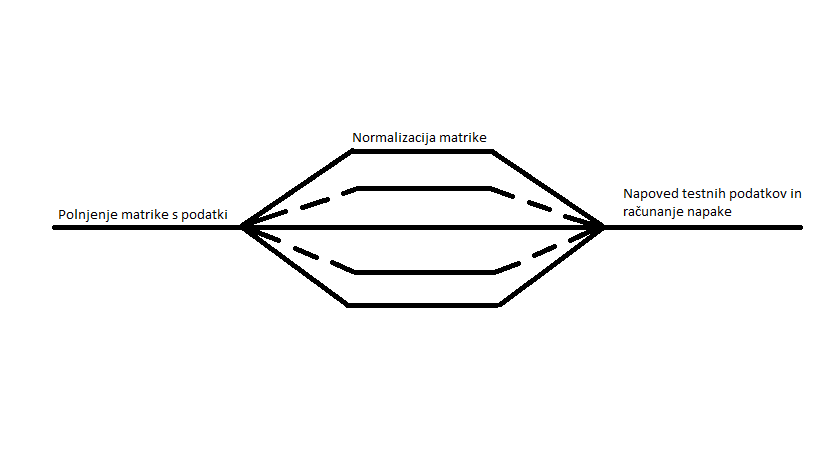
\includegraphics[scale=0.6]{Shema.png}
\label{shema}
\end{center}
\end{figure}


\subsection{Meritve}
Za vsako velikost problema (število dimenzij in stanj v matriki) se je opravilo 22 meritev. V tabeli~\ref{tab1} so prikazani rezultati, ko je program uporabljal 2 niti za paralelizacijo. V tabeli ~\ref{tab2} je program deloval na osmih, v tabeli ~\ref{tab3} pa na šestnajstih. Skupno se je torej opravilo 1056 meritev.

\begin{table}[H]
\caption{Povprečni časi meritev pri paralelizaciji z dvemi nitmi. Stolpci predstavljajo število dimenzij, vrstice pa število stanj. Časovna enota je sekunda.}
\label{tab1}
\begin{center}
\begin{tabular}{p{2cm} p{2cm}   p{1.5cm}|p{1.5cm}|p{1.5cm}|p{1.5cm}|}
& & \multicolumn{4}{ c }{Dimenzije} \\ \cline{3-5}
 && \cellcolor[gray]{0.9} 7 & \cellcolor[gray]{0.9} 6 & \cellcolor[gray]{0.9} 5 & \cellcolor[gray]{0.9} 4 \\ \cline{3-6}
\multirow{4}{*}{Stanja} 
&\cellcolor[gray]{0.9} 20 & 6,13 & 1,43 & 0,99 & 0,88 \\ \cline{2-6}
&\cellcolor[gray]{0.9} 16 & 2,72 & 1,43 & 1 & 0,93 \\ \cline{2-6}
&\cellcolor[gray]{0.9} 12 & 1,55 & 1,09 & 0,96 & 0,88 \\ \cline{2-6}
&\cellcolor[gray]{0.9} 8 & 1,18 & 0,96 & 0.9 & 0,89 \\ \cline{2-6}
\end{tabular}
\end{center}
\end{table}

\begin{table}[H]
\caption{Povprečni časi meritev pri paralelizaciji z osmimi nitmi. Stolpci predstavljajo število dimenzij, vrstice pa število stanj. Časovna enota je sekunda.}
\label{tab2}
\begin{center}
\begin{tabular}{p{2cm} p{2cm}   p{1.5cm}|p{1.5cm}|p{1.5cm}|p{1.5cm}|}
& & \multicolumn{4}{ c }{Dimenzije} \\ \cline{3-5}
 && \cellcolor[gray]{0.9} 7 & \cellcolor[gray]{0.9} 6 & \cellcolor[gray]{0.9} 5 & \cellcolor[gray]{0.9} 4 \\ \cline{3-6}
\multirow{4}{*}{Stanja} 
&\cellcolor[gray]{0.9} 20 & 2,81 & 1,24 & 0,98 & 0,91  \\ \cline{2-6}
&\cellcolor[gray]{0.9} 16 & 2,11 & 1,35 & 1,01 & 0,9  \\ \cline{2-6}
&\cellcolor[gray]{0.9} 12 & 1,46 & 1,13 & 0,94 & 0,91  \\ \cline{2-6}
&\cellcolor[gray]{0.9} 8 &  1,2 & 0,99 & 0,91 & 0,86  \\ \cline{2-6}
\end{tabular}
\end{center}
\end{table}

\begin{table}[H]
\caption{Povprečni časi meritev pri paralelizaciji s šestnajstimi nitmi. Stolpci predstavljajo število dimenzij, vrstice pa število stanj. Časovna enota je sekunda.}
\label{tab3}
\begin{center}
\begin{tabular}{p{2cm} p{2cm}   p{1.5cm}|p{1.5cm}|p{1.5cm}|p{1.5cm}|}
& & \multicolumn{4}{ c }{Dimenzije} \\ \cline{3-5}
 && \cellcolor[gray]{0.9} 7 & \cellcolor[gray]{0.9} 6 & \cellcolor[gray]{0.9} 5 & \cellcolor[gray]{0.9} 4 \\ \cline{3-6}
\multirow{4}{*}{Stanja} 
&\cellcolor[gray]{0.9} 20 & 2,39 & 1,23 & 0,98 & 0,9  \\ \cline{2-6}
&\cellcolor[gray]{0.9} 16 & 2,01 & 1,38 & 1,02 & 0,94 \\ \cline{2-6}
&\cellcolor[gray]{0.9} 12 & 1,45 & 1,13 & 0,98 & 0,95  \\ \cline{2-6}
&\cellcolor[gray]{0.9} 8  & 0,99 & 1    & 0,91 & 0,88 \\ \cline{2-6}
\end{tabular}
\end{center}
\end{table}



\subsection{Analiza meritev}

Pohitritev je izračunana na največji matriki iz meritev. Torej vsebuje 20 stanj in 7 dimenzij. V tabeli ~\ref{analiza1} so podani rezultati. Z rezultati sva zadovoljna, saj sva dosegla določeno pohitritev. Največja pohitritev je pri programu z 12 nitmi, kar je kar malo presenečenje, saj se je analiza izvajala na procesorju Ryzen 1700, ki podpira do 16 niti. Ker so podatki o hitrosti povprečje tridesetih ponovitev, je največja verjetnost, da razlogi tičijo v strojni opremi. Iz tabele je tudi lepo razvidno, da učinkovitost z večjim številom niti pada. 

\begin{table}[H]
\caption{Prikaz pohitritev in učinkovitosti algoritmov, ko delujejo pri različnim številom niti}
\label{analiza1}
\begin{center}
\begin{tabular}{|p{2cm}| p{2cm} | p{2cm}| p{2cm}| }
 \hline
\cellcolor[gray]{0.9} Število niti &\cellcolor[gray]{0.9}  Povprečni čas [s] & \cellcolor[gray]{0.9}  Pohitritev & \cellcolor[gray]{0.9}  Učinkovitost \\ \hline
1 & 8,74 & 1 & 1 \\ \hline
2 & 6,13 & 1,42 & 0,713 \\ \hline
4 & 3,40 & 2,56 & 0,64 \\ \hline
6 & 2,82 & 3,09 & 0,52 \\ \hline
12 & 2,23 & 3,93 & 0,33 \\ \hline
16 & 2,25 & 3,88 & 0,24 \\ \hline
\end{tabular}
\end{center}
\end{table}

\begin{figure}[H]
\begin{center}
\caption{Prikaz pohitritev in učinkovitosti algoritmov.}
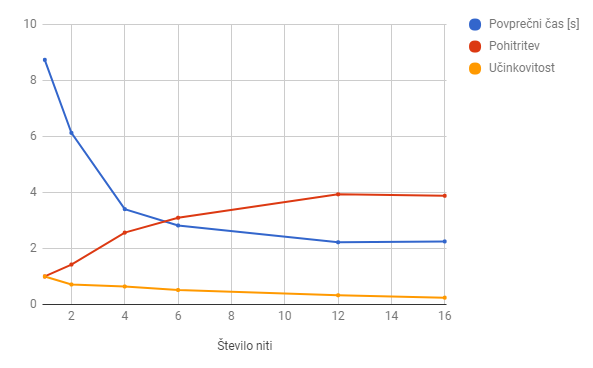
\includegraphics[scale=1]{GrafUcinkovitost.png}
\label{grafOpenMP}
\end{center}
\end{figure}


\section{Paralelizacija z OpenMP}
Ideja paralelizacije tudi s programskim vmesnikom OpenMP ostaja enaka \ref{shema}. Potrebno je bilo le paziti katere spremenljivke so skupne vsem nitim, katere pa morajo biti privatne. Na koncu sva ugotovila, da sta privatni spremenljivki trenutni seštevek vseh vrednosti v stolpcu in pa spremenljivka, ki služi kot števec indeksa za željeno celico v matriki. Ostale spremenljivke so skupne vsem nitim.

\subsection{Meritve}
Za vsako kombinacijo dimenzij in stanj se je zopet opravilo 22 meritev. V tabeli ~\ref{tab4} so prikazani vsi rezultati programa z OpenMP vmesnikom. Za boljšo vizualno predstavitev podatkov je dodan tudi graf \ref{grafOpenMP}.

\begin{table}[H]
\caption{Povprečni časi meritev pri paralelizaciji z OpenMP. Stolpci predstavljajo število dimenzij, vrstice pa število stanj. Časovna enota je sekunda.}
\label{tab4}
\begin{center}
\begin{tabular}{p{2cm} p{2cm}   p{1.5cm}|p{1.5cm}|p{1.5cm}|p{1.5cm}|}
& & \multicolumn{4}{ c }{Dimenzije} \\ \cline{3-5}
 && \cellcolor[gray]{0.9} 7 & \cellcolor[gray]{0.9} 6 & \cellcolor[gray]{0.9} 5 & \cellcolor[gray]{0.9} 4 \\ \cline{3-6}
\multirow{4}{*}{Stanja} 
&\cellcolor[gray]{0.9} 20 & 2,13 & 1,01 & 0,85 & 0,78 \\ \cline{2-6}
&\cellcolor[gray]{0.9} 16 & 1,86 & 1,1 & 0,88 & 0,79 \\ \cline{2-6}
&\cellcolor[gray]{0.9} 12 & 1,25 & 0,98 & 0,83 & 0,76  \\ \cline{2-6}
&\cellcolor[gray]{0.9} 8 & 0,98 & 0,84 & 0,76 & 0,73  \\ \cline{2-6}
\end{tabular}
\end{center}
\end{table}


\begin{figure}[H]
\begin{center}
\caption{Časovna zahtevnost za različno število korakov. Barve premic določajo število stanj, kot je opisano v legendi.}
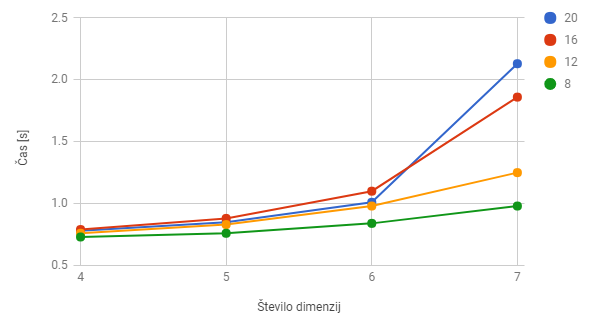
\includegraphics[scale=1]{GrafOpenMP.png}
\label{grafOpenMP}
\end{center}
\end{figure}



\end{document}
